\documentclass[1p]{elsarticle_modified}
%\bibliographystyle{elsarticle-num}

%\usepackage[colorlinks]{hyperref}
%\usepackage{abbrmath_seonhwa} %\Abb, \Ascr, \Acal ,\Abf, \Afrak
\usepackage{amsfonts}
\usepackage{amssymb}
\usepackage{amsmath}
\usepackage{amsthm}
\usepackage{scalefnt}
\usepackage{amsbsy}
\usepackage{kotex}
\usepackage{caption}
\usepackage{subfig}
\usepackage{color}
\usepackage{graphicx}
\usepackage{xcolor} %% white, black, red, green, blue, cyan, magenta, yellow
\usepackage{float}
\usepackage{setspace}
\usepackage{hyperref}

\usepackage{tikz}
\usetikzlibrary{arrows}

\usepackage{multirow}
\usepackage{array} % fixed length table
\usepackage{hhline}

%%%%%%%%%%%%%%%%%%%%%
\makeatletter
\renewcommand*\env@matrix[1][\arraystretch]{%
	\edef\arraystretch{#1}%
	\hskip -\arraycolsep
	\let\@ifnextchar\new@ifnextchar
	\array{*\c@MaxMatrixCols c}}
\makeatother %https://tex.stackexchange.com/questions/14071/how-can-i-increase-the-line-spacing-in-a-matrix
%%%%%%%%%%%%%%%

\usepackage[normalem]{ulem}

\newcommand{\msout}[1]{\ifmmode\text{\sout{\ensuremath{#1}}}\else\sout{#1}\fi}
%SOURCE: \msout is \stkout macro in https://tex.stackexchange.com/questions/20609/strikeout-in-math-mode

\newcommand{\cancel}[1]{
	\ifmmode
	{\color{red}\msout{#1}}
	\else
	{\color{red}\sout{#1}}
	\fi
}

\newcommand{\add}[1]{
	{\color{blue}\uwave{#1}}
}

\newcommand{\replace}[2]{
	\ifmmode
	{\color{red}\msout{#1}}{\color{blue}\uwave{#2}}
	\else
	{\color{red}\sout{#1}}{\color{blue}\uwave{#2}}
	\fi
}

\newcommand{\Sol}{\mathcal{S}} %segment
\newcommand{\D}{D} %diagram
\newcommand{\A}{\mathcal{A}} %arc


%%%%%%%%%%%%%%%%%%%%%%%%%%%%%5 test

\def\sl{\operatorname{\textup{SL}}(2,\Cbb)}
\def\psl{\operatorname{\textup{PSL}}(2,\Cbb)}
\def\quan{\mkern 1mu \triangleright \mkern 1mu}

\theoremstyle{definition}
\newtheorem{thm}{Theorem}[section]
\newtheorem{prop}[thm]{Proposition}
\newtheorem{lem}[thm]{Lemma}
\newtheorem{ques}[thm]{Question}
\newtheorem{cor}[thm]{Corollary}
\newtheorem{defn}[thm]{Definition}
\newtheorem{exam}[thm]{Example}
\newtheorem{rmk}[thm]{Remark}
\newtheorem{alg}[thm]{Algorithm}

\newcommand{\I}{\sqrt{-1}}
\begin{document}

%\begin{frontmatter}
%
%\title{Boundary parabolic representations of knots up to 8 crossings}
%
%%% Group authors per affiliation:
%\author{Yunhi Cho} 
%\address{Department of Mathematics, University of Seoul, Seoul, Korea}
%\ead{yhcho@uos.ac.kr}
%
%
%\author{Seonhwa Kim} %\fnref{s_kim}}
%\address{Center for Geometry and Physics, Institute for Basic Science, Pohang, 37673, Korea}
%\ead{ryeona17@ibs.re.kr}
%
%\author{Hyuk Kim}
%\address{Department of Mathematical Sciences, Seoul National University, Seoul 08826, Korea}
%\ead{hyukkim@snu.ac.kr}
%
%\author{Seokbeom Yoon}
%\address{Department of Mathematical Sciences, Seoul National University, Seoul, 08826,  Korea}
%\ead{sbyoon15@snu.ac.kr}
%
%\begin{abstract}
%We find all boundary parabolic representation of knots up to 8 crossings.
%
%\end{abstract}
%\begin{keyword}
%    \MSC[2010] 57M25 
%\end{keyword}
%
%\end{frontmatter}

%\linenumbers
%\tableofcontents
%
\newcommand\colored[1]{\textcolor{white}{\rule[-0.35ex]{0.8em}{1.4ex}}\kern-0.8em\color{red} #1}%
%\newcommand\colored[1]{\textcolor{white}{ #1}\kern-2.17ex	\textcolor{white}{ #1}\kern-1.81ex	\textcolor{white}{ #1}\kern-2.15ex\color{red}#1	}

{\Large $\underline{12n_{0643}~(K12n_{0643})}$}

\setlength{\tabcolsep}{10pt}
\renewcommand{\arraystretch}{1.6}
\vspace{1cm}\begin{tabular}{m{100pt}>{\centering\arraybackslash}m{274pt}}
\multirow{5}{120pt}{
	\centering
	\includegraphics[width=112pt]{../../../GIT/diagram.site/Diagrams/png/2732_12n_0643.png}\\
\ \ \ A knot diagram\footnotemark}&
\allowdisplaybreaks
\textbf{Linearized knot diagam} \\
\cline{2-2}
 &
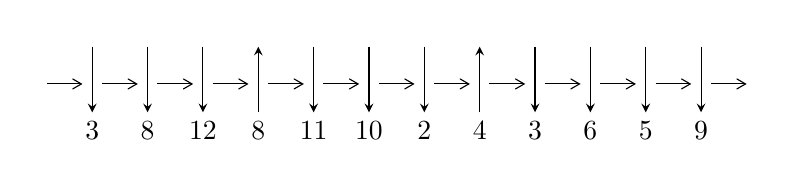
\begin{tikzpicture}[x=20pt, y=17pt]
	% nodes
	\node (C0) at (0, 0) {};
	\node (C1) at (1, 0) {};
	\node (C1U) at (1, +1) {};
	\node (C1D) at (1, -1) {3};

	\node (C2) at (2, 0) {};
	\node (C2U) at (2, +1) {};
	\node (C2D) at (2, -1) {8};

	\node (C3) at (3, 0) {};
	\node (C3U) at (3, +1) {};
	\node (C3D) at (3, -1) {12};

	\node (C4) at (4, 0) {};
	\node (C4U) at (4, +1) {};
	\node (C4D) at (4, -1) {8};

	\node (C5) at (5, 0) {};
	\node (C5U) at (5, +1) {};
	\node (C5D) at (5, -1) {11};

	\node (C6) at (6, 0) {};
	\node (C6U) at (6, +1) {};
	\node (C6D) at (6, -1) {10};

	\node (C7) at (7, 0) {};
	\node (C7U) at (7, +1) {};
	\node (C7D) at (7, -1) {2};

	\node (C8) at (8, 0) {};
	\node (C8U) at (8, +1) {};
	\node (C8D) at (8, -1) {4};

	\node (C9) at (9, 0) {};
	\node (C9U) at (9, +1) {};
	\node (C9D) at (9, -1) {3};

	\node (C10) at (10, 0) {};
	\node (C10U) at (10, +1) {};
	\node (C10D) at (10, -1) {6};

	\node (C11) at (11, 0) {};
	\node (C11U) at (11, +1) {};
	\node (C11D) at (11, -1) {5};

	\node (C12) at (12, 0) {};
	\node (C12U) at (12, +1) {};
	\node (C12D) at (12, -1) {9};
	\node (C13) at (13, 0) {};

	% arrows
	\draw[->,>={angle 60}]
	(C0) edge (C1) (C1) edge (C2) (C2) edge (C3) (C3) edge (C4) (C4) edge (C5) (C5) edge (C6) (C6) edge (C7) (C7) edge (C8) (C8) edge (C9) (C9) edge (C10) (C10) edge (C11) (C11) edge (C12) (C12) edge (C13) ;	\draw[->,>=stealth]
	(C1U) edge (C1D) (C2U) edge (C2D) (C3U) edge (C3D) (C4D) edge (C4U) (C5U) edge (C5D) (C6U) edge (C6D) (C7U) edge (C7D) (C8D) edge (C8U) (C9U) edge (C9D) (C10U) edge (C10D) (C11U) edge (C11D) (C12U) edge (C12D) ;
	\end{tikzpicture} \\
\hhline{~~} \\& 
\textbf{Solving Sequence} \\ \cline{2-2} 
 &
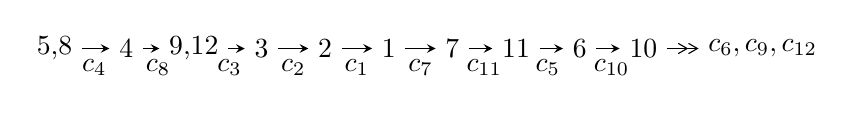
\begin{tikzpicture}[x=23pt, y=7pt]
	% node
	\node (A0) at (-1/8, 0) {5,8};
	\node (A1) at (1, 0) {4};
	\node (A2) at (33/16, 0) {9,12};
	\node (A3) at (25/8, 0) {3};
	\node (A4) at (33/8, 0) {2};
	\node (A5) at (41/8, 0) {1};
	\node (A6) at (49/8, 0) {7};
	\node (A7) at (57/8, 0) {11};
	\node (A8) at (65/8, 0) {6};
	\node (A9) at (73/8, 0) {10};
	\node (C1) at (1/2, -1) {$c_{4}$};
	\node (C2) at (3/2, -1) {$c_{8}$};
	\node (C3) at (21/8, -1) {$c_{3}$};
	\node (C4) at (29/8, -1) {$c_{2}$};
	\node (C5) at (37/8, -1) {$c_{1}$};
	\node (C6) at (45/8, -1) {$c_{7}$};
	\node (C7) at (53/8, -1) {$c_{11}$};
	\node (C8) at (61/8, -1) {$c_{5}$};
	\node (C9) at (69/8, -1) {$c_{10}$};
	\node (A10) at (11, 0) {$c_{6},c_{9},c_{12}$};

	% edge
	\draw[->,>=stealth]	
	(A0) edge (A1) (A1) edge (A2) (A2) edge (A3) (A3) edge (A4) (A4) edge (A5) (A5) edge (A6) (A6) edge (A7) (A7) edge (A8) (A8) edge (A9) ;
	\draw[->>,>={angle 60}]	
	(A9) edge (A10);
\end{tikzpicture} \\ 

\end{tabular} \\

\footnotetext{
The image of knot diagram is generated by the software ``\textbf{Draw programme}" developed by Andrew Bartholomew(\url{http://www.layer8.co.uk/maths/draw/index.htm\#Running-draw}), where we modified some parts for our purpose(\url{https://github.com/CATsTAILs/LinksPainter}).
}\phantom \\ \newline 
\centering \textbf{Ideals for irreducible components\footnotemark of $X_{\text{par}}$} 
 
\begin{align*}
I^u_{1}&=\langle 
-68009 u^{16}-44301 u^{15}+\cdots+147102 b+345073,\;a-1,\;u^{17}+9 u^{15}+\cdots+2 u+1\rangle \\
I^u_{2}&=\langle 
-2 u^5-5 u^4+13 u^2+34 b+15 u-21,\;59 u^5+122 u^4+187 u^3+135 u^2+34 a+25 u+628,\\
\phantom{I^u_{2}}&\phantom{= \langle  }u^6+2 u^5+3 u^4+2 u^3+10 u-1\rangle \\
I^u_{3}&=\langle 
-42 u^{10}-15 u^9-68 u^8-63 u^7-114 u^6-63 u^5+35 u^4+150 u^3+89 u^2+23 b+116 u+25,\;a+1,\\
\phantom{I^u_{3}}&\phantom{= \langle  }u^{11}+2 u^9+u^8+3 u^7+u^6-3 u^4- u^3-4 u^2-1\rangle \\
I^u_{4}&=\langle 
-6 u^{11}-5 u^{10}+48 u^9-118 u^8+124 u^7-211 u^6-246 u^5-51 u^4-750 u^3+85 u^2+236 b-746 u-12,\\
\phantom{I^u_{4}}&\phantom{= \langle  }65 u^{11}-585 u^{10}+\cdots+472 a-5416,\\
\phantom{I^u_{4}}&\phantom{= \langle  }u^{12}-5 u^{11}+15 u^{10}-32 u^9+58 u^8-77 u^7+103 u^6-93 u^5+100 u^4-55 u^3+48 u^2-12 u+8\rangle \\
\\
\end{align*}
\raggedright * 4 irreducible components of $\dim_{\mathbb{C}}=0$, with total 46 representations.\\
\footnotetext{All coefficients of polynomials are rational numbers. But the coefficients are sometimes approximated in decimal forms when there is not enough margin.}
\newpage
\renewcommand{\arraystretch}{1}
\centering \section*{I. $I^u_{1}= \langle -6.80\times10^{4} u^{16}-4.43\times10^{4} u^{15}+\cdots+1.47\times10^{5} b+3.45\times10^{5},\;a-1,\;u^{17}+9 u^{15}+\cdots+2 u+1 \rangle$}
\flushleft \textbf{(i) Arc colorings}\\
\begin{tabular}{m{7pt} m{180pt} m{7pt} m{180pt} }
\flushright $a_{5}=$&$\begin{pmatrix}1\\0\end{pmatrix}$ \\
\flushright $a_{8}=$&$\begin{pmatrix}0\\u\end{pmatrix}$ \\
\flushright $a_{4}=$&$\begin{pmatrix}1\\u^2\end{pmatrix}$ \\
\flushright $a_{9}=$&$\begin{pmatrix}u\\u^3+u\end{pmatrix}$ \\
\flushright $a_{12}=$&$\begin{pmatrix}1\\0.462325 u^{16}+0.301158 u^{15}+\cdots-5.67284 u-2.34581\end{pmatrix}$ \\
\flushright $a_{3}=$&$\begin{pmatrix}-0.462325 u^{16}-0.301158 u^{15}+\cdots+5.67284 u+3.34581\\-0.287392 u^{16}+0.502305 u^{15}+\cdots-1.98646 u-0.919770\end{pmatrix}$ \\
\flushright $a_{2}=$&$\begin{pmatrix}-0.462325 u^{16}-0.301158 u^{15}+\cdots+5.67284 u+3.34581\\-0.279955 u^{16}+0.529707 u^{15}+\cdots-3.05110 u-1.22093\end{pmatrix}$ \\
\flushright $a_{1}=$&$\begin{pmatrix}-0.00743702 u^{16}-0.0274028 u^{15}+\cdots+1.06464 u+1.30116\\0.190147 u^{16}+0.239167 u^{15}+\cdots-4.54595 u-2.01725\end{pmatrix}$ \\
\flushright $a_{7}=$&$\begin{pmatrix}-1.13202 u^{16}-0.272111 u^{15}+\cdots+8.20193 u+0.644696\\0.0817596 u^{16}-0.0818956 u^{15}+\cdots+1.62497 u+0.308167\end{pmatrix}$ \\
\flushright $a_{11}=$&$\begin{pmatrix}0.462325 u^{16}+0.301158 u^{15}+\cdots-5.67284 u-1.34581\\0.462325 u^{16}+0.301158 u^{15}+\cdots-5.67284 u-2.34581\end{pmatrix}$ \\
\flushright $a_{6}=$&$\begin{pmatrix}0.757155 u^{16}-0.173743 u^{15}+\cdots-4.75102 u-0.727196\\0.294829 u^{16}-0.474902 u^{15}+\cdots+0.921816 u+0.618612\end{pmatrix}$ \\
\flushright $a_{10}=$&$\begin{pmatrix}1.21378 u^{16}+0.190215 u^{15}+\cdots-6.57697 u-0.336528\\0.456629 u^{16}+0.363958 u^{15}+\cdots-1.82594 u+0.390668\end{pmatrix}$\\&\end{tabular}
\flushleft \textbf{(ii) Obstruction class $= -1$}\\~\\
\flushleft \textbf{(iii) Cusp Shapes $= -\frac{173298}{24517} u^{16}-\frac{19700}{24517} u^{15}+\cdots+\frac{1212498}{24517} u-\frac{66405}{24517}$}\\~\\
\newpage\renewcommand{\arraystretch}{1}
\flushleft \textbf{(iv) u-Polynomials at the component}\newline \\
\begin{tabular}{m{50pt}|m{274pt}}
Crossings & \hspace{64pt}u-Polynomials at each crossing \\
\hline $$\begin{aligned}c_{1}\end{aligned}$$&$\begin{aligned}
&u^{17}+25 u^{16}+\cdots-5 u+1
\end{aligned}$\\
\hline $$\begin{aligned}c_{2},c_{7},c_{12}\end{aligned}$$&$\begin{aligned}
&u^{17}+u^{16}+\cdots+u+1
\end{aligned}$\\
\hline $$\begin{aligned}c_{3}\end{aligned}$$&$\begin{aligned}
&u^{17}-11 u^{16}+\cdots-48 u+8
\end{aligned}$\\
\hline $$\begin{aligned}c_{4},c_{8}\end{aligned}$$&$\begin{aligned}
&u^{17}+9 u^{15}+\cdots+2 u+1
\end{aligned}$\\
\hline $$\begin{aligned}c_{5},c_{6},c_{10}\\c_{11}\end{aligned}$$&$\begin{aligned}
&u^{17}+7 u^{16}+\cdots+72 u+8
\end{aligned}$\\
\hline $$\begin{aligned}c_{9}\end{aligned}$$&$\begin{aligned}
&u^{17}-20 u^{15}+\cdots+194 u+259
\end{aligned}$\\
\hline
\end{tabular}\\~\\
\newpage\renewcommand{\arraystretch}{1}
\flushleft \textbf{(v) Riley Polynomials at the component}\newline \\
\begin{tabular}{m{50pt}|m{274pt}}
Crossings & \hspace{64pt}Riley Polynomials at each crossing \\
\hline $$\begin{aligned}c_{1}\end{aligned}$$&$\begin{aligned}
&y^{17}-65 y^{16}+\cdots+87 y-1
\end{aligned}$\\
\hline $$\begin{aligned}c_{2},c_{7},c_{12}\end{aligned}$$&$\begin{aligned}
&y^{17}-25 y^{16}+\cdots-5 y-1
\end{aligned}$\\
\hline $$\begin{aligned}c_{3}\end{aligned}$$&$\begin{aligned}
&y^{17}+3 y^{16}+\cdots+672 y-64
\end{aligned}$\\
\hline $$\begin{aligned}c_{4},c_{8}\end{aligned}$$&$\begin{aligned}
&y^{17}+18 y^{16}+\cdots+20 y-1
\end{aligned}$\\
\hline $$\begin{aligned}c_{5},c_{6},c_{10}\\c_{11}\end{aligned}$$&$\begin{aligned}
&y^{17}+19 y^{16}+\cdots+288 y-64
\end{aligned}$\\
\hline $$\begin{aligned}c_{9}\end{aligned}$$&$\begin{aligned}
&y^{17}-40 y^{16}+\cdots-96526 y-67081
\end{aligned}$\\
\hline
\end{tabular}\\~\\
\newpage\flushleft \textbf{(vi) Complex Volumes and Cusp Shapes}
$$\begin{array}{c|c|c}  
\text{Solutions to }I^u_{1}& \I (\text{vol} + \sqrt{-1}CS) & \text{Cusp shape}\\
 \hline 
\begin{aligned}
u &= \phantom{-}0.273982 + 1.067890 I \\
a &= \phantom{-}1.00000\phantom{ +0.000000I} \\
b &= -0.476176 + 0.479879 I\end{aligned}
 & -0.94573 + 1.67377 I & -6.92989 - 3.16143 I \\ \hline\begin{aligned}
u &= \phantom{-}0.273982 - 1.067890 I \\
a &= \phantom{-}1.00000\phantom{ +0.000000I} \\
b &= -0.476176 - 0.479879 I\end{aligned}
 & -0.94573 - 1.67377 I & -6.92989 + 3.16143 I \\ \hline\begin{aligned}
u &= \phantom{-}0.124569 + 1.229950 I \\
a &= \phantom{-}1.00000\phantom{ +0.000000I} \\
b &= -0.37277 + 1.64716 I\end{aligned}
 & -5.40408 + 3.79366 I & -9.42026 - 1.67014 I \\ \hline\begin{aligned}
u &= \phantom{-}0.124569 - 1.229950 I \\
a &= \phantom{-}1.00000\phantom{ +0.000000I} \\
b &= -0.37277 - 1.64716 I\end{aligned}
 & -5.40408 - 3.79366 I & -9.42026 + 1.67014 I \\ \hline\begin{aligned}
u &= -0.747531 + 1.177200 I \\
a &= \phantom{-}1.00000\phantom{ +0.000000I} \\
b &= -0.11531 - 1.52558 I\end{aligned}
 & \phantom{-}5.74347 - 3.70748 I & -0.330584 + 0.385083 I \\ \hline\begin{aligned}
u &= -0.747531 - 1.177200 I \\
a &= \phantom{-}1.00000\phantom{ +0.000000I} \\
b &= -0.11531 + 1.52558 I\end{aligned}
 & \phantom{-}5.74347 + 3.70748 I & -0.330584 - 0.385083 I \\ \hline\begin{aligned}
u &= \phantom{-}0.18378 + 1.48034 I \\
a &= \phantom{-}1.00000\phantom{ +0.000000I} \\
b &= -0.958979 - 0.657777 I\end{aligned}
 & -12.88920 + 1.26003 I & -11.26337 - 0.06200 I \\ \hline\begin{aligned}
u &= \phantom{-}0.18378 - 1.48034 I \\
a &= \phantom{-}1.00000\phantom{ +0.000000I} \\
b &= -0.958979 + 0.657777 I\end{aligned}
 & -12.88920 - 1.26003 I & -11.26337 + 0.06200 I \\ \hline\begin{aligned}
u &= -0.435602 + 0.235065 I \\
a &= \phantom{-}1.00000\phantom{ +0.000000I} \\
b &= \phantom{-}0.02738 - 1.68451 I\end{aligned}
 & \phantom{-}10.39050 - 1.51785 I & \phantom{-}0.08130 + 5.70683 I \\ \hline\begin{aligned}
u &= -0.435602 - 0.235065 I \\
a &= \phantom{-}1.00000\phantom{ +0.000000I} \\
b &= \phantom{-}0.02738 + 1.68451 I\end{aligned}
 & \phantom{-}10.39050 + 1.51785 I & \phantom{-}0.08130 - 5.70683 I\\
 \hline 
 \end{array}$$\newpage$$\begin{array}{c|c|c}  
\text{Solutions to }I^u_{1}& \I (\text{vol} + \sqrt{-1}CS) & \text{Cusp shape}\\
 \hline 
\begin{aligned}
u &= \phantom{-}0.438102 + 0.020053 I \\
a &= \phantom{-}1.00000\phantom{ +0.000000I} \\
b &= -0.092822 + 0.789763 I\end{aligned}
 & \phantom{-}1.61479 + 1.53966 I & -1.79490 - 4.96374 I \\ \hline\begin{aligned}
u &= \phantom{-}0.438102 - 0.020053 I \\
a &= \phantom{-}1.00000\phantom{ +0.000000I} \\
b &= -0.092822 - 0.789763 I\end{aligned}
 & \phantom{-}1.61479 - 1.53966 I & -1.79490 + 4.96374 I \\ \hline\begin{aligned}
u &= -0.52463 + 1.57423 I \\
a &= \phantom{-}1.00000\phantom{ +0.000000I} \\
b &= -0.970536 - 0.552496 I\end{aligned}
 & -13.1856 - 7.5502 I & -11.07949 + 4.57676 I \\ \hline\begin{aligned}
u &= -0.52463 - 1.57423 I \\
a &= \phantom{-}1.00000\phantom{ +0.000000I} \\
b &= -0.970536 + 0.552496 I\end{aligned}
 & -13.1856 + 7.5502 I & -11.07949 - 4.57676 I \\ \hline\begin{aligned}
u &= -0.314233\phantom{ +0.000000I} \\
a &= \phantom{-}1.00000\phantom{ +0.000000I} \\
b &= -0.331071\phantom{ +0.000000I}\end{aligned}
 & -0.707107\phantom{ +0.000000I} & -14.3070\phantom{ +0.000000I} \\ \hline\begin{aligned}
u &= \phantom{-}0.84444 + 1.52914 I \\
a &= \phantom{-}1.00000\phantom{ +0.000000I} \\
b &= -0.37526 + 1.57337 I\end{aligned}
 & -6.35474 + 12.51650 I & -8.10916 - 5.80852 I \\ \hline\begin{aligned}
u &= \phantom{-}0.84444 - 1.52914 I \\
a &= \phantom{-}1.00000\phantom{ +0.000000I} \\
b &= -0.37526 - 1.57337 I\end{aligned}
 & -6.35474 - 12.51650 I & -8.10916 + 5.80852 I\\
 \hline 
 \end{array}$$\newpage\newpage\renewcommand{\arraystretch}{1}
\centering \section*{II. $I^u_{2}= \langle -2 u^5-5 u^4+13 u^2+34 b+15 u-21,\;59 u^5+122 u^4+\cdots+34 a+628,\;u^6+2 u^5+3 u^4+2 u^3+10 u-1 \rangle$}
\flushleft \textbf{(i) Arc colorings}\\
\begin{tabular}{m{7pt} m{180pt} m{7pt} m{180pt} }
\flushright $a_{5}=$&$\begin{pmatrix}1\\0\end{pmatrix}$ \\
\flushright $a_{8}=$&$\begin{pmatrix}0\\u\end{pmatrix}$ \\
\flushright $a_{4}=$&$\begin{pmatrix}1\\u^2\end{pmatrix}$ \\
\flushright $a_{9}=$&$\begin{pmatrix}u\\u^3+u\end{pmatrix}$ \\
\flushright $a_{12}=$&$\begin{pmatrix}-1.73529 u^{5}-3.58824 u^{4}+\cdots-0.735294 u-18.4706\\0.0588235 u^{5}+0.147059 u^{4}+\cdots-0.441176 u+0.617647\end{pmatrix}$ \\
\flushright $a_{3}=$&$\begin{pmatrix}1.47059 u^{5}+3.17647 u^{4}+\cdots+0.470588 u+14.9412\\0.0588235 u^{5}+0.147059 u^{4}+\cdots-0.441176 u-0.382353\end{pmatrix}$ \\
\flushright $a_{2}=$&$\begin{pmatrix}1.47059 u^{5}+3.17647 u^{4}+\cdots+0.470588 u+14.9412\\-0.0588235 u^{5}-0.147059 u^{4}+\cdots+0.441176 u-0.617647\end{pmatrix}$ \\
\flushright $a_{1}=$&$\begin{pmatrix}-1.82353 u^{5}-4.05882 u^{4}+\cdots-0.823529 u-18.6471\\0.323529 u^{5}+0.0588235 u^{4}+\cdots+2.32353 u+0.147059\end{pmatrix}$ \\
\flushright $a_{7}=$&$\begin{pmatrix}2.23529 u^{5}+4.58824 u^{4}+\cdots+0.235294 u+22.4706\\-0.117647 u^{5}-0.294118 u^{4}+\cdots-0.117647 u-0.735294\end{pmatrix}$ \\
\flushright $a_{11}=$&$\begin{pmatrix}-1.67647 u^{5}-3.44118 u^{4}+\cdots-1.17647 u-17.8529\\0.0588235 u^{5}+0.147059 u^{4}+\cdots-0.441176 u+0.617647\end{pmatrix}$ \\
\flushright $a_{6}=$&$\begin{pmatrix}-0.882353 u^{5}-1.70588 u^{4}+\cdots+0.117647 u-9.26471\\0.176471 u^{5}+0.441176 u^{4}+\cdots-0.323529 u+0.352941\end{pmatrix}$ \\
\flushright $a_{10}=$&$\begin{pmatrix}-2.35294 u^{5}-4.88235 u^{4}+\cdots-0.352941 u-23.2059\\0.117647 u^{5}+0.294118 u^{4}+\cdots+0.117647 u+0.735294\end{pmatrix}$\\&\end{tabular}
\flushleft \textbf{(ii) Obstruction class $= -1$}\\~\\
\flushleft \textbf{(iii) Cusp Shapes $= -\frac{16}{17} u^5-\frac{40}{17} u^4-4 u^3-\frac{100}{17} u^2-\frac{16}{17} u-\frac{338}{17}$}\\~\\
\newpage\renewcommand{\arraystretch}{1}
\flushleft \textbf{(iv) u-Polynomials at the component}\newline \\
\begin{tabular}{m{50pt}|m{274pt}}
Crossings & \hspace{64pt}u-Polynomials at each crossing \\
\hline $$\begin{aligned}c_{1}\end{aligned}$$&$\begin{aligned}
&u^6+6 u^5+5 u^4-14 u^3+26 u^2+144 u+121
\end{aligned}$\\
\hline $$\begin{aligned}c_{2},c_{7},c_{12}\end{aligned}$$&$\begin{aligned}
&u^6+2 u^5- u^4+2 u^2-10 u-11
\end{aligned}$\\
\hline $$\begin{aligned}c_{3}\end{aligned}$$&$\begin{aligned}
&(u^3+u^2-1)^2
\end{aligned}$\\
\hline $$\begin{aligned}c_{4},c_{8}\end{aligned}$$&$\begin{aligned}
&u^6+2 u^5+3 u^4+2 u^3+10 u-1
\end{aligned}$\\
\hline $$\begin{aligned}c_{5},c_{6},c_{10}\\c_{11}\end{aligned}$$&$\begin{aligned}
&(u^3- u^2+2 u-1)^2
\end{aligned}$\\
\hline $$\begin{aligned}c_{9}\end{aligned}$$&$\begin{aligned}
&u^6+5 u^5+4 u^4-11 u^3-14 u^2-8
\end{aligned}$\\
\hline
\end{tabular}\\~\\
\newpage\renewcommand{\arraystretch}{1}
\flushleft \textbf{(v) Riley Polynomials at the component}\newline \\
\begin{tabular}{m{50pt}|m{274pt}}
Crossings & \hspace{64pt}Riley Polynomials at each crossing \\
\hline $$\begin{aligned}c_{1}\end{aligned}$$&$\begin{aligned}
&y^6-26 y^5+245 y^4-1422 y^3+5918 y^2-14444 y+14641
\end{aligned}$\\
\hline $$\begin{aligned}c_{2},c_{7},c_{12}\end{aligned}$$&$\begin{aligned}
&y^6-6 y^5+5 y^4+14 y^3+26 y^2-144 y+121
\end{aligned}$\\
\hline $$\begin{aligned}c_{3}\end{aligned}$$&$\begin{aligned}
&(y^3- y^2+2 y-1)^2
\end{aligned}$\\
\hline $$\begin{aligned}c_{4},c_{8}\end{aligned}$$&$\begin{aligned}
&y^6+2 y^5+y^4-46 y^3-46 y^2-100 y+1
\end{aligned}$\\
\hline $$\begin{aligned}c_{5},c_{6},c_{10}\\c_{11}\end{aligned}$$&$\begin{aligned}
&(y^3+3 y^2+2 y-1)^2
\end{aligned}$\\
\hline $$\begin{aligned}c_{9}\end{aligned}$$&$\begin{aligned}
&y^6-17 y^5+98 y^4-249 y^3+132 y^2+224 y+64
\end{aligned}$\\
\hline
\end{tabular}\\~\\
\newpage\flushleft \textbf{(vi) Complex Volumes and Cusp Shapes}
$$\begin{array}{c|c|c}  
\text{Solutions to }I^u_{2}& \I (\text{vol} + \sqrt{-1}CS) & \text{Cusp shape}\\
 \hline 
\begin{aligned}
u &= \phantom{-}0.714259 + 0.979949 I \\
a &= -1.55592 - 0.28013 I \\
b &= \phantom{-}0.215080 - 1.307140 I\end{aligned}
 & \phantom{-}1.11345 + 5.65624 I & -6.98049 - 5.95889 I \\ \hline\begin{aligned}
u &= \phantom{-}0.714259 - 0.979949 I \\
a &= -1.55592 + 0.28013 I \\
b &= \phantom{-}0.215080 + 1.307140 I\end{aligned}
 & \phantom{-}1.11345 - 5.65624 I & -6.98049 + 5.95889 I \\ \hline\begin{aligned}
u &= -1.85465\phantom{ +0.000000I} \\
a &= -0.0537944\phantom{ +0.000000I} \\
b &= \phantom{-}0.569840\phantom{ +0.000000I}\end{aligned}
 & -7.16171\phantom{ +0.000000I} & -20.0390\phantom{ +0.000000I} \\ \hline\begin{aligned}
u &= \phantom{-}0.0997696\phantom{ +0.000000I} \\
a &= -18.5893\phantom{ +0.000000I} \\
b &= \phantom{-}0.569840\phantom{ +0.000000I}\end{aligned}
 & -7.16171\phantom{ +0.000000I} & -20.0390\phantom{ +0.000000I} \\ \hline\begin{aligned}
u &= -0.83682 + 1.72481 I \\
a &= -0.622526 - 0.112080 I \\
b &= \phantom{-}0.215080 + 1.307140 I\end{aligned}
 & \phantom{-}1.11345 - 5.65624 I & -6.98049 + 5.95889 I \\ \hline\begin{aligned}
u &= -0.83682 - 1.72481 I \\
a &= -0.622526 + 0.112080 I \\
b &= \phantom{-}0.215080 - 1.307140 I\end{aligned}
 & \phantom{-}1.11345 + 5.65624 I & -6.98049 - 5.95889 I\\
 \hline 
 \end{array}$$\newpage\newpage\renewcommand{\arraystretch}{1}
\centering \section*{III. $I^u_{3}= \langle -42 u^{10}-15 u^9+\cdots+23 b+25,\;a+1,\;u^{11}+2 u^9+u^8+3 u^7+u^6-3 u^4- u^3-4 u^2-1 \rangle$}
\flushleft \textbf{(i) Arc colorings}\\
\begin{tabular}{m{7pt} m{180pt} m{7pt} m{180pt} }
\flushright $a_{5}=$&$\begin{pmatrix}1\\0\end{pmatrix}$ \\
\flushright $a_{8}=$&$\begin{pmatrix}0\\u\end{pmatrix}$ \\
\flushright $a_{4}=$&$\begin{pmatrix}1\\u^2\end{pmatrix}$ \\
\flushright $a_{9}=$&$\begin{pmatrix}u\\u^3+u\end{pmatrix}$ \\
\flushright $a_{12}=$&$\begin{pmatrix}-1\\1.82609 u^{10}+0.652174 u^{9}+\cdots-5.04348 u-1.08696\end{pmatrix}$ \\
\flushright $a_{3}=$&$\begin{pmatrix}1.82609 u^{10}+0.652174 u^{9}+\cdots-5.04348 u-0.0869565\\1.13043 u^{10}-0.739130 u^{9}+\cdots-2.21739 u+3.56522\end{pmatrix}$ \\
\flushright $a_{2}=$&$\begin{pmatrix}1.82609 u^{10}+0.652174 u^{9}+\cdots-5.04348 u-0.0869565\\1.82609 u^{10}-0.347826 u^{9}+\cdots-4.04348 u+2.91304\end{pmatrix}$ \\
\flushright $a_{1}=$&$\begin{pmatrix}0.695652 u^{10}+0.391304 u^{9}+\cdots-1.82609 u-1.65217\\2.30435 u^{10}+0.608696 u^{9}+\cdots-6.17391 u-1.34783\end{pmatrix}$ \\
\flushright $a_{7}=$&$\begin{pmatrix}1.65217 u^{10}-0.695652 u^{9}+\cdots-4.08696 u+1.82609\\1.08696 u^{10}-1.82609 u^{9}+\cdots-0.478261 u+5.04348\end{pmatrix}$ \\
\flushright $a_{11}=$&$\begin{pmatrix}1.82609 u^{10}+0.652174 u^{9}+\cdots-5.04348 u-2.08696\\1.82609 u^{10}+0.652174 u^{9}+\cdots-5.04348 u-1.08696\end{pmatrix}$ \\
\flushright $a_{6}=$&$\begin{pmatrix}-2.26087 u^{10}+0.478261 u^{9}+\cdots+5.43478 u-2.13043\\-0.434783 u^{10}+1.13043 u^{9}+\cdots+0.391304 u-4.21739\end{pmatrix}$ \\
\flushright $a_{10}=$&$\begin{pmatrix}-0.565217 u^{10}-1.13043 u^{9}+\cdots+3.60870 u+3.21739\\-2.82609 u^{10}-0.652174 u^{9}+\cdots+9.04348 u+1.08696\end{pmatrix}$\\&\end{tabular}
\flushleft \textbf{(ii) Obstruction class $= 1$}\\~\\
\flushleft \textbf{(iii) Cusp Shapes $= -\frac{31}{23} u^{10}+\frac{7}{23} u^9-\frac{48}{23} u^8+\frac{11}{23} u^7-\frac{71}{23} u^6+\frac{34}{23} u^5+\frac{91}{23} u^4+\frac{137}{23} u^3-\frac{17}{23} u^2+\frac{21}{23} u-\frac{257}{23}$}\\~\\
\newpage\renewcommand{\arraystretch}{1}
\flushleft \textbf{(iv) u-Polynomials at the component}\newline \\
\begin{tabular}{m{50pt}|m{274pt}}
Crossings & \hspace{64pt}u-Polynomials at each crossing \\
\hline $$\begin{aligned}c_{1}\end{aligned}$$&$\begin{aligned}
&u^{11}-11 u^{10}+\cdots+7 u-1
\end{aligned}$\\
\hline $$\begin{aligned}c_{2}\end{aligned}$$&$\begin{aligned}
&u^{11}+u^{10}-5 u^9-5 u^8+9 u^7+8 u^6-8 u^5-7 u^4+4 u^3+3 u^2- u-1
\end{aligned}$\\
\hline $$\begin{aligned}c_{3}\end{aligned}$$&$\begin{aligned}
&u^{11}+4 u^{10}+10 u^9+16 u^8+16 u^7+7 u^6-3 u^5-5 u^4+2 u^2-1
\end{aligned}$\\
\hline $$\begin{aligned}c_{4}\end{aligned}$$&$\begin{aligned}
&u^{11}+2 u^9+u^8+3 u^7+u^6-3 u^4- u^3-4 u^2-1
\end{aligned}$\\
\hline $$\begin{aligned}c_{5},c_{6}\end{aligned}$$&$\begin{aligned}
&u^{11}+8 u^9+23 u^7+28 u^5+u^4+12 u^3+3 u^2+1
\end{aligned}$\\
\hline $$\begin{aligned}c_{7},c_{12}\end{aligned}$$&$\begin{aligned}
&u^{11}- u^{10}-5 u^9+5 u^8+9 u^7-8 u^6-8 u^5+7 u^4+4 u^3-3 u^2- u+1
\end{aligned}$\\
\hline $$\begin{aligned}c_{8}\end{aligned}$$&$\begin{aligned}
&u^{11}+2 u^9- u^8+3 u^7- u^6+3 u^4- u^3+4 u^2+1
\end{aligned}$\\
\hline $$\begin{aligned}c_{9}\end{aligned}$$&$\begin{aligned}
&u^{11}-5 u^9-2 u^8+4 u^7+9 u^6+5 u^5-2 u^4-13 u^3+7 u^2+2 u+1
\end{aligned}$\\
\hline $$\begin{aligned}c_{10},c_{11}\end{aligned}$$&$\begin{aligned}
&u^{11}+8 u^9+23 u^7+28 u^5- u^4+12 u^3-3 u^2-1
\end{aligned}$\\
\hline
\end{tabular}\\~\\
\newpage\renewcommand{\arraystretch}{1}
\flushleft \textbf{(v) Riley Polynomials at the component}\newline \\
\begin{tabular}{m{50pt}|m{274pt}}
Crossings & \hspace{64pt}Riley Polynomials at each crossing \\
\hline $$\begin{aligned}c_{1}\end{aligned}$$&$\begin{aligned}
&y^{11}-15 y^{10}+\cdots-13 y-1
\end{aligned}$\\
\hline $$\begin{aligned}c_{2},c_{7},c_{12}\end{aligned}$$&$\begin{aligned}
&y^{11}-11 y^{10}+\cdots+7 y-1
\end{aligned}$\\
\hline $$\begin{aligned}c_{3}\end{aligned}$$&$\begin{aligned}
&y^{11}+4 y^{10}+\cdots+4 y-1
\end{aligned}$\\
\hline $$\begin{aligned}c_{4},c_{8}\end{aligned}$$&$\begin{aligned}
&y^{11}+4 y^{10}+\cdots-8 y-1
\end{aligned}$\\
\hline $$\begin{aligned}c_{5},c_{6},c_{10}\\c_{11}\end{aligned}$$&$\begin{aligned}
&y^{11}+16 y^{10}+\cdots-6 y-1
\end{aligned}$\\
\hline $$\begin{aligned}c_{9}\end{aligned}$$&$\begin{aligned}
&y^{11}-10 y^{10}+\cdots-10 y-1
\end{aligned}$\\
\hline
\end{tabular}\\~\\
\newpage\flushleft \textbf{(vi) Complex Volumes and Cusp Shapes}
$$\begin{array}{c|c|c}  
\text{Solutions to }I^u_{3}& \I (\text{vol} + \sqrt{-1}CS) & \text{Cusp shape}\\
 \hline 
\begin{aligned}
u &= \phantom{-}1.02184\phantom{ +0.000000I} \\
a &= -1.00000\phantom{ +0.000000I} \\
b &= -0.445195\phantom{ +0.000000I}\end{aligned}
 & -6.47878\phantom{ +0.000000I} & -5.43850\phantom{ +0.000000I} \\ \hline\begin{aligned}
u &= -0.960985 + 0.510912 I \\
a &= -1.00000\phantom{ +0.000000I} \\
b &= -0.233007 + 1.358440 I\end{aligned}
 & -1.89567 + 2.51034 I & -5.23089 - 0.60579 I \\ \hline\begin{aligned}
u &= -0.960985 - 0.510912 I \\
a &= -1.00000\phantom{ +0.000000I} \\
b &= -0.233007 - 1.358440 I\end{aligned}
 & -1.89567 - 2.51034 I & -5.23089 + 0.60579 I \\ \hline\begin{aligned}
u &= \phantom{-}0.062554 + 0.872739 I \\
a &= -1.00000\phantom{ +0.000000I} \\
b &= \phantom{-}0.166908 + 0.916041 I\end{aligned}
 & \phantom{-}0.12106 + 1.89765 I & -8.02738 - 3.63931 I \\ \hline\begin{aligned}
u &= \phantom{-}0.062554 - 0.872739 I \\
a &= -1.00000\phantom{ +0.000000I} \\
b &= \phantom{-}0.166908 - 0.916041 I\end{aligned}
 & \phantom{-}0.12106 - 1.89765 I & -8.02738 + 3.63931 I \\ \hline\begin{aligned}
u &= -0.448669 + 1.127200 I \\
a &= -1.00000\phantom{ +0.000000I} \\
b &= \phantom{-}0.193075 + 0.390923 I\end{aligned}
 & -1.65984 - 3.19570 I & -7.07775 + 5.40642 I \\ \hline\begin{aligned}
u &= -0.448669 - 1.127200 I \\
a &= -1.00000\phantom{ +0.000000I} \\
b &= \phantom{-}0.193075 - 0.390923 I\end{aligned}
 & -1.65984 + 3.19570 I & -7.07775 - 5.40642 I \\ \hline\begin{aligned}
u &= \phantom{-}0.065465 + 0.570358 I \\
a &= -1.00000\phantom{ +0.000000I} \\
b &= \phantom{-}0.02836 - 1.73242 I\end{aligned}
 & \phantom{-}9.80306 - 1.15540 I & -10.75281 - 0.76912 I \\ \hline\begin{aligned}
u &= \phantom{-}0.065465 - 0.570358 I \\
a &= -1.00000\phantom{ +0.000000I} \\
b &= \phantom{-}0.02836 + 1.73242 I\end{aligned}
 & \phantom{-}9.80306 + 1.15540 I & -10.75281 + 0.76912 I \\ \hline\begin{aligned}
u &= \phantom{-}0.77071 + 1.27691 I \\
a &= -1.00000\phantom{ +0.000000I} \\
b &= \phantom{-}0.06726 - 1.54442 I\end{aligned}
 & \phantom{-}5.09546 + 4.16451 I & -9.19190 - 5.51053 I\\
 \hline 
 \end{array}$$\newpage$$\begin{array}{c|c|c}  
\text{Solutions to }I^u_{3}& \I (\text{vol} + \sqrt{-1}CS) & \text{Cusp shape}\\
 \hline 
\begin{aligned}
u &= \phantom{-}0.77071 - 1.27691 I \\
a &= -1.00000\phantom{ +0.000000I} \\
b &= \phantom{-}0.06726 + 1.54442 I\end{aligned}
 & \phantom{-}5.09546 - 4.16451 I & -9.19190 + 5.51053 I\\
 \hline 
 \end{array}$$\newpage\newpage\renewcommand{\arraystretch}{1}
\centering \section*{IV. $I^u_{4}= \langle -6 u^{11}-5 u^{10}+\cdots+236 b-12,\;65 u^{11}-585 u^{10}+\cdots+472 a-5416,\;u^{12}-5 u^{11}+\cdots-12 u+8 \rangle$}
\flushleft \textbf{(i) Arc colorings}\\
\begin{tabular}{m{7pt} m{180pt} m{7pt} m{180pt} }
\flushright $a_{5}=$&$\begin{pmatrix}1\\0\end{pmatrix}$ \\
\flushright $a_{8}=$&$\begin{pmatrix}0\\u\end{pmatrix}$ \\
\flushright $a_{4}=$&$\begin{pmatrix}1\\u^2\end{pmatrix}$ \\
\flushright $a_{9}=$&$\begin{pmatrix}u\\u^3+u\end{pmatrix}$ \\
\flushright $a_{12}=$&$\begin{pmatrix}-0.137712 u^{11}+1.23941 u^{10}+\cdots-19.0805 u+11.4746\\0.0254237 u^{11}+0.0211864 u^{10}+\cdots+3.16102 u+0.0508475\end{pmatrix}$ \\
\flushright $a_{3}=$&$\begin{pmatrix}0.502119 u^{11}-2.51907 u^{10}+\cdots+13.3051 u-3.74576\\-0.555085 u^{11}+2.74576 u^{10}+\cdots-8.43220 u+0.389831\end{pmatrix}$ \\
\flushright $a_{2}=$&$\begin{pmatrix}0.502119 u^{11}-2.51907 u^{10}+\cdots+13.3051 u-3.74576\\-0.338983 u^{11}+1.80085 u^{10}+\cdots-4.31356 u+0.322034\end{pmatrix}$ \\
\flushright $a_{1}=$&$\begin{pmatrix}-0.252119 u^{11}+1.76907 u^{10}+\cdots-15.5551 u+9.74576\\0.0805085 u^{11}-0.224576 u^{10}+\cdots+7.09322 u-1.33898\end{pmatrix}$ \\
\flushright $a_{7}=$&$\begin{pmatrix}-0.646186 u^{11}+3.56568 u^{10}+\cdots-20.8008 u+7.95763\\-0.00423729 u^{11}+0.0381356 u^{10}+\cdots+2.38983 u+0.491525\end{pmatrix}$ \\
\flushright $a_{11}=$&$\begin{pmatrix}-0.112288 u^{11}+1.26059 u^{10}+\cdots-15.9195 u+11.5254\\0.0254237 u^{11}+0.0211864 u^{10}+\cdots+3.16102 u+0.0508475\end{pmatrix}$ \\
\flushright $a_{6}=$&$\begin{pmatrix}1.18432 u^{11}-5.65890 u^{10}+\cdots+17.5424 u+4.11864\\0.0296610 u^{11}-0.0169492 u^{10}+\cdots+0.771186 u-1.44068\end{pmatrix}$ \\
\flushright $a_{10}=$&$\begin{pmatrix}0.641949 u^{11}-3.52754 u^{10}+\cdots+23.1907 u-7.46610\\0.00423729 u^{11}-0.0381356 u^{10}+\cdots-2.38983 u-0.491525\end{pmatrix}$\\&\end{tabular}
\flushleft \textbf{(ii) Obstruction class $= -1$}\\~\\
\flushleft \textbf{(iii) Cusp Shapes $= \frac{4}{59} u^{11}-\frac{95}{59} u^{10}+\frac{440}{59} u^9-21 u^8+\frac{2474}{59} u^7-\frac{4068}{59} u^6+\frac{4884}{59} u^5-\frac{5807}{59} u^4+\frac{4512}{59} u^3-\frac{4344}{59} u^2+\frac{1638}{59} u-\frac{1762}{59}$}\\~\\
\newpage\renewcommand{\arraystretch}{1}
\flushleft \textbf{(iv) u-Polynomials at the component}\newline \\
\begin{tabular}{m{50pt}|m{274pt}}
Crossings & \hspace{64pt}u-Polynomials at each crossing \\
\hline $$\begin{aligned}c_{1}\end{aligned}$$&$\begin{aligned}
&u^{12}+15 u^{11}+\cdots+96 u+64
\end{aligned}$\\
\hline $$\begin{aligned}c_{2},c_{7},c_{12}\end{aligned}$$&$\begin{aligned}
&u^{12}-3 u^{11}+\cdots-8 u+8
\end{aligned}$\\
\hline $$\begin{aligned}c_{3}\end{aligned}$$&$\begin{aligned}
&(u^3+u^2-1)^4
\end{aligned}$\\
\hline $$\begin{aligned}c_{4},c_{8}\end{aligned}$$&$\begin{aligned}
&u^{12}-5 u^{11}+\cdots-12 u+8
\end{aligned}$\\
\hline $$\begin{aligned}c_{5},c_{6},c_{10}\\c_{11}\end{aligned}$$&$\begin{aligned}
&(u^3- u^2+2 u-1)^4
\end{aligned}$\\
\hline $$\begin{aligned}c_{9}\end{aligned}$$&$\begin{aligned}
&u^{12}-6 u^{11}+\cdots+18 u+59
\end{aligned}$\\
\hline
\end{tabular}\\~\\
\newpage\renewcommand{\arraystretch}{1}
\flushleft \textbf{(v) Riley Polynomials at the component}\newline \\
\begin{tabular}{m{50pt}|m{274pt}}
Crossings & \hspace{64pt}Riley Polynomials at each crossing \\
\hline $$\begin{aligned}c_{1}\end{aligned}$$&$\begin{aligned}
&y^{12}-15 y^{11}+\cdots-18944 y+4096
\end{aligned}$\\
\hline $$\begin{aligned}c_{2},c_{7},c_{12}\end{aligned}$$&$\begin{aligned}
&y^{12}-15 y^{11}+\cdots-96 y+64
\end{aligned}$\\
\hline $$\begin{aligned}c_{3}\end{aligned}$$&$\begin{aligned}
&(y^3- y^2+2 y-1)^4
\end{aligned}$\\
\hline $$\begin{aligned}c_{4},c_{8}\end{aligned}$$&$\begin{aligned}
&y^{12}+5 y^{11}+\cdots+624 y+64
\end{aligned}$\\
\hline $$\begin{aligned}c_{5},c_{6},c_{10}\\c_{11}\end{aligned}$$&$\begin{aligned}
&(y^3+3 y^2+2 y-1)^4
\end{aligned}$\\
\hline $$\begin{aligned}c_{9}\end{aligned}$$&$\begin{aligned}
&y^{12}-16 y^{11}+\cdots-8820 y+3481
\end{aligned}$\\
\hline
\end{tabular}\\~\\
\newpage\flushleft \textbf{(vi) Complex Volumes and Cusp Shapes}
$$\begin{array}{c|c|c}  
\text{Solutions to }I^u_{4}& \I (\text{vol} + \sqrt{-1}CS) & \text{Cusp shape}\\
 \hline 
\begin{aligned}
u &= \phantom{-}0.044973 + 0.916855 I \\
a &= -1.22501 - 0.79096 I \\
b &= \phantom{-}0.215080 + 1.307140 I\end{aligned}
 & \phantom{-}1.11345\phantom{ +0.000000I} & -6.98049 + 0. I\phantom{ +0.000000I} \\ \hline\begin{aligned}
u &= \phantom{-}0.044973 - 0.916855 I \\
a &= -1.22501 + 0.79096 I \\
b &= \phantom{-}0.215080 - 1.307140 I\end{aligned}
 & \phantom{-}1.11345\phantom{ +0.000000I} & -6.98049 + 0. I\phantom{ +0.000000I} \\ \hline\begin{aligned}
u &= -0.404600 + 1.033930 I \\
a &= -1.272350 + 0.353092 I \\
b &= \phantom{-}0.569840\phantom{ +0.000000I}\end{aligned}
 & -3.02413 - 2.82812 I & -13.50976 + 2.97945 I \\ \hline\begin{aligned}
u &= -0.404600 - 1.033930 I \\
a &= -1.272350 - 0.353092 I \\
b &= \phantom{-}0.569840\phantom{ +0.000000I}\end{aligned}
 & -3.02413 + 2.82812 I & -13.50976 - 2.97945 I \\ \hline\begin{aligned}
u &= \phantom{-}0.670107 + 1.158730 I \\
a &= -0.576131 - 0.371997 I \\
b &= \phantom{-}0.215080 - 1.307140 I\end{aligned}
 & \phantom{-}1.11345\phantom{ +0.000000I} & -6.98049 + 0. I\phantom{ +0.000000I} \\ \hline\begin{aligned}
u &= \phantom{-}0.670107 - 1.158730 I \\
a &= -0.576131 + 0.371997 I \\
b &= \phantom{-}0.215080 + 1.307140 I\end{aligned}
 & \phantom{-}1.11345\phantom{ +0.000000I} & -6.98049 + 0. I\phantom{ +0.000000I} \\ \hline\begin{aligned}
u &= \phantom{-}0.076727 + 0.622517 I \\
a &= \phantom{-}2.13780 - 2.88995 I \\
b &= \phantom{-}0.215080 + 1.307140 I\end{aligned}
 & -3.02413 - 2.82812 I & -13.50976 + 2.97945 I \\ \hline\begin{aligned}
u &= \phantom{-}0.076727 - 0.622517 I \\
a &= \phantom{-}2.13780 + 2.88995 I \\
b &= \phantom{-}0.215080 - 1.307140 I\end{aligned}
 & -3.02413 + 2.82812 I & -13.50976 - 2.97945 I \\ \hline\begin{aligned}
u &= \phantom{-}0.14972 + 1.45838 I \\
a &= -0.729747 + 0.202513 I \\
b &= \phantom{-}0.569840\phantom{ +0.000000I}\end{aligned}
 & -3.02413 + 2.82812 I & -13.50976 - 2.97945 I \\ \hline\begin{aligned}
u &= \phantom{-}0.14972 - 1.45838 I \\
a &= -0.729747 - 0.202513 I \\
b &= \phantom{-}0.569840\phantom{ +0.000000I}\end{aligned}
 & -3.02413 - 2.82812 I & -13.50976 + 2.97945 I\\
 \hline 
 \end{array}$$\newpage$$\begin{array}{c|c|c}  
\text{Solutions to }I^u_{4}& \I (\text{vol} + \sqrt{-1}CS) & \text{Cusp shape}\\
 \hline 
\begin{aligned}
u &= \phantom{-}1.96307 + 1.10908 I \\
a &= \phantom{-}0.165439 + 0.223646 I \\
b &= \phantom{-}0.215080 + 1.307140 I\end{aligned}
 & -3.02413 - 2.82812 I & -13.50976 + 2.97945 I \\ \hline\begin{aligned}
u &= \phantom{-}1.96307 - 1.10908 I \\
a &= \phantom{-}0.165439 - 0.223646 I \\
b &= \phantom{-}0.215080 - 1.307140 I\end{aligned}
 & -3.02413 + 2.82812 I & -13.50976 - 2.97945 I\\
 \hline 
 \end{array}$$\newpage
\newpage\renewcommand{\arraystretch}{1}
\centering \section*{ V. u-Polynomials}
\begin{tabular}{m{50pt}|m{274pt}}
Crossings & \hspace{64pt}u-Polynomials at each crossing \\
\hline $$\begin{aligned}c_{1}\end{aligned}$$&$\begin{aligned}
&(u^6+6 u^5+5 u^4-14 u^3+26 u^2+144 u+121)\\
&\cdot(u^{11}-11 u^{10}+\cdots+7 u-1)(u^{12}+15 u^{11}+\cdots+96 u+64)\\
&\cdot(u^{17}+25 u^{16}+\cdots-5 u+1)
\end{aligned}$\\
\hline $$\begin{aligned}c_{2}\end{aligned}$$&$\begin{aligned}
&(u^6+2 u^5- u^4+2 u^2-10 u-11)\\
&\cdot(u^{11}+u^{10}-5 u^9-5 u^8+9 u^7+8 u^6-8 u^5-7 u^4+4 u^3+3 u^2- u-1)\\
&\cdot(u^{12}-3 u^{11}+\cdots-8 u+8)(u^{17}+u^{16}+\cdots+u+1)
\end{aligned}$\\
\hline $$\begin{aligned}c_{3}\end{aligned}$$&$\begin{aligned}
&(u^3+u^2-1)^6\\
&\cdot(u^{11}+4 u^{10}+10 u^9+16 u^8+16 u^7+7 u^6-3 u^5-5 u^4+2 u^2-1)\\
&\cdot(u^{17}-11 u^{16}+\cdots-48 u+8)
\end{aligned}$\\
\hline $$\begin{aligned}c_{4}\end{aligned}$$&$\begin{aligned}
&(u^6+2 u^5+3 u^4+2 u^3+10 u-1)\\
&\cdot(u^{11}+2 u^9+u^8+3 u^7+u^6-3 u^4- u^3-4 u^2-1)\\
&\cdot(u^{12}-5 u^{11}+\cdots-12 u+8)(u^{17}+9 u^{15}+\cdots+2 u+1)
\end{aligned}$\\
\hline $$\begin{aligned}c_{5},c_{6}\end{aligned}$$&$\begin{aligned}
&(u^3- u^2+2 u-1)^6(u^{11}+8 u^9+23 u^7+28 u^5+u^4+12 u^3+3 u^2+1)\\
&\cdot(u^{17}+7 u^{16}+\cdots+72 u+8)
\end{aligned}$\\
\hline $$\begin{aligned}c_{7},c_{12}\end{aligned}$$&$\begin{aligned}
&(u^6+2 u^5- u^4+2 u^2-10 u-11)\\
&\cdot(u^{11}- u^{10}-5 u^9+5 u^8+9 u^7-8 u^6-8 u^5+7 u^4+4 u^3-3 u^2- u+1)\\
&\cdot(u^{12}-3 u^{11}+\cdots-8 u+8)(u^{17}+u^{16}+\cdots+u+1)
\end{aligned}$\\
\hline $$\begin{aligned}c_{8}\end{aligned}$$&$\begin{aligned}
&(u^6+2 u^5+3 u^4+2 u^3+10 u-1)\\
&\cdot(u^{11}+2 u^9- u^8+3 u^7- u^6+3 u^4- u^3+4 u^2+1)\\
&\cdot(u^{12}-5 u^{11}+\cdots-12 u+8)(u^{17}+9 u^{15}+\cdots+2 u+1)
\end{aligned}$\\
\hline $$\begin{aligned}c_{9}\end{aligned}$$&$\begin{aligned}
&(u^6+5 u^5+4 u^4-11 u^3-14 u^2-8)\\
&\cdot(u^{11}-5 u^9-2 u^8+4 u^7+9 u^6+5 u^5-2 u^4-13 u^3+7 u^2+2 u+1)\\
&\cdot(u^{12}-6 u^{11}+\cdots+18 u+59)(u^{17}-20 u^{15}+\cdots+194 u+259)
\end{aligned}$\\
\hline $$\begin{aligned}c_{10},c_{11}\end{aligned}$$&$\begin{aligned}
&(u^3- u^2+2 u-1)^6(u^{11}+8 u^9+23 u^7+28 u^5- u^4+12 u^3-3 u^2-1)\\
&\cdot(u^{17}+7 u^{16}+\cdots+72 u+8)
\end{aligned}$\\
\hline
\end{tabular}\newpage\renewcommand{\arraystretch}{1}
\centering \section*{ VI. Riley Polynomials}
\begin{tabular}{m{50pt}|m{274pt}}
Crossings & \hspace{64pt}Riley Polynomials at each crossing \\
\hline $$\begin{aligned}c_{1}\end{aligned}$$&$\begin{aligned}
&(y^6-26 y^5+245 y^4-1422 y^3+5918 y^2-14444 y+14641)\\
&\cdot(y^{11}-15 y^{10}+\cdots-13 y-1)(y^{12}-15 y^{11}+\cdots-18944 y+4096)\\
&\cdot(y^{17}-65 y^{16}+\cdots+87 y-1)
\end{aligned}$\\
\hline $$\begin{aligned}c_{2},c_{7},c_{12}\end{aligned}$$&$\begin{aligned}
&(y^6-6 y^5+5 y^4+14 y^3+26 y^2-144 y+121)\\
&\cdot(y^{11}-11 y^{10}+\cdots+7 y-1)(y^{12}-15 y^{11}+\cdots-96 y+64)\\
&\cdot(y^{17}-25 y^{16}+\cdots-5 y-1)
\end{aligned}$\\
\hline $$\begin{aligned}c_{3}\end{aligned}$$&$\begin{aligned}
&((y^3- y^2+2 y-1)^6)(y^{11}+4 y^{10}+\cdots+4 y-1)\\
&\cdot(y^{17}+3 y^{16}+\cdots+672 y-64)
\end{aligned}$\\
\hline $$\begin{aligned}c_{4},c_{8}\end{aligned}$$&$\begin{aligned}
&(y^6+2 y^5+\cdots-100 y+1)(y^{11}+4 y^{10}+\cdots-8 y-1)\\
&\cdot(y^{12}+5 y^{11}+\cdots+624 y+64)(y^{17}+18 y^{16}+\cdots+20 y-1)
\end{aligned}$\\
\hline $$\begin{aligned}c_{5},c_{6},c_{10}\\c_{11}\end{aligned}$$&$\begin{aligned}
&((y^3+3 y^2+2 y-1)^6)(y^{11}+16 y^{10}+\cdots-6 y-1)\\
&\cdot(y^{17}+19 y^{16}+\cdots+288 y-64)
\end{aligned}$\\
\hline $$\begin{aligned}c_{9}\end{aligned}$$&$\begin{aligned}
&(y^6-17 y^5+98 y^4-249 y^3+132 y^2+224 y+64)\\
&\cdot(y^{11}-10 y^{10}+\cdots-10 y-1)(y^{12}-16 y^{11}+\cdots-8820 y+3481)\\
&\cdot(y^{17}-40 y^{16}+\cdots-96526 y-67081)
\end{aligned}$\\
\hline
\end{tabular}
\vskip 2pc
\end{document}